% This file was converted to LaTeX by Writer2LaTeX ver. 1.0.2
% see http://writer2latex.sourceforge.net for more info
\documentclass[twoside,letterpaper]{article}
\usepackage[latin1]{inputenc}
\usepackage[T1]{fontenc}
\usepackage[english]{babel}
\usepackage{amsmath}
\usepackage{amssymb,amsfonts,textcomp}
\usepackage{color}
\usepackage{array}
\usepackage{supertabular}
\usepackage{hhline}
\usepackage{hyperref}
\hypersetup{pdftex, colorlinks=true, linkcolor=blue, citecolor=blue, filecolor=blue, urlcolor=blue, pdftitle=SYSTEM AND SOFTWARE ARCHITECTURAL AND DETAILED DESIGN DESCRIPTION, pdfauthor=Clinton Jeffery, pdfsubject=, pdfkeywords=}
\usepackage[pdftex]{graphicx}
% Outline numbering
\setcounter{secnumdepth}{5}
\renewcommand\thesection{\arabic{section}}
\renewcommand\thesubsection{\arabic{section}.\arabic{subsection}}
\renewcommand\thesubsubsection{\arabic{section}.\arabic{subsection}.\arabic{subsubsection}}
\renewcommand\theparagraph{\arabic{section}.\arabic{subsection}.\arabic{subsubsection}.\arabic{paragraph}}
\renewcommand\thesubparagraph{\arabic{section}.\arabic{subsection}.\arabic{subsubsection}.\arabic{paragraph}.\arabic{subparagraph}}
\makeatletter
\newcommand\arraybslash{\let\\\@arraycr}
\makeatother
% List styles
\newcommand\liststyleWWviiiNumii{%
\renewcommand\theenumi{\arabic{enumi}}
\renewcommand\theenumii{\arabic{enumii}}
\renewcommand\theenumiii{\arabic{enumiii}}
\renewcommand\theenumiv{\arabic{enumiv}}
\renewcommand\labelenumi{\theenumi)}
\renewcommand\labelenumii{\theenumii.}
\renewcommand\labelenumiii{\theenumiii.}
\renewcommand\labelenumiv{\theenumiv.}
}
% Page layout (geometry)
\setlength\voffset{-1in}
\setlength\hoffset{-1in}
\setlength\topmargin{0.5in}
\setlength\oddsidemargin{1in}
\setlength\evensidemargin{1in}
\setlength\textheight{8.278in}
\setlength\textwidth{6.5in}
\setlength\footskip{0.561in}
\setlength\headheight{0.5in}
\setlength\headsep{0.461in}
% Footnote rule
\setlength{\skip\footins}{0.0469in}
\renewcommand\footnoterule{\vspace*{-0.0071in}\setlength\leftskip{0pt}\setlength\rightskip{0pt plus 1fil}\noindent\textcolor{black}{\rule{0.25\columnwidth}{0.0071in}}\vspace*{0.0398in}}
% Pages styles
\makeatletter
\newcommand\ps@Standard{
  \renewcommand\@oddhead{}
  \renewcommand\@evenhead{\@oddhead}
  \renewcommand\@oddfoot{\foreignlanguage{english}{\textcolor{black}{\hfill SSDD Page }}{\textcolor{black}{\thepage{}}}}
  \renewcommand\@evenfoot{\@oddfoot}
  \renewcommand\thepage{\arabic{page}}
}
\newcommand\ps@Convertix{
  \renewcommand\@oddhead{}
  \renewcommand\@evenhead{\@oddhead}
  \renewcommand\@oddfoot{}
  \renewcommand\@evenfoot{\@oddfoot}
  \renewcommand\thepage{\arabic{page}}
}
\newcommand\ps@Convertviii{
  \renewcommand\@oddhead{}
  \renewcommand\@evenhead{\@oddhead}
  \renewcommand\@oddfoot{}
  \renewcommand\@evenfoot{\@oddfoot}
  \renewcommand\thepage{\arabic{page}}
}
\newcommand\ps@Convertvii{
  \renewcommand\@oddhead{}
  \renewcommand\@evenhead{\@oddhead}
  \renewcommand\@oddfoot{}
  \renewcommand\@evenfoot{\@oddfoot}
  \renewcommand\thepage{\arabic{page}}
}
\newcommand\ps@Convertvi{
  \renewcommand\@oddhead{}
  \renewcommand\@evenhead{\@oddhead}
  \renewcommand\@oddfoot{}
  \renewcommand\@evenfoot{\@oddfoot}
  \renewcommand\thepage{\arabic{page}}
}
\newcommand\ps@Convertiv{
  \renewcommand\@oddhead{}
  \renewcommand\@evenhead{\@oddhead}
  \renewcommand\@oddfoot{}
  \renewcommand\@evenfoot{\@oddfoot}
  \renewcommand\thepage{\arabic{page}}
}
\newcommand\ps@FirstPage{
  \renewcommand\@oddhead{}
  \renewcommand\@evenhead{\@oddhead}
  \renewcommand\@oddfoot{\foreignlanguage{english}{\textcolor{black}{\hfill SSDD Page }}
{\textcolor{black}{\thepage{}}}}
  \renewcommand\@evenfoot{\@oddfoot}
  \renewcommand\thepage{\arabic{page}}
}
\makeatother
\pagestyle{Standard}
\setlength\tabcolsep{1mm}
\renewcommand\arraystretch{1.3}
\title{SYSTEM AND SOFTWARE ARCHITECTURAL AND DETAILED DESIGN DESCRIPTION}
\author{Python Team}
\date{2013-12-19}

% % % % % % % % % % % % % % %
% Place my packages here    %
% % % % % % % % % % % % % % %

% New tables
\usepackage[utf8]{inputenc}
\usepackage{tabularx}
\usepackage{ragged2e}
\usepackage{booktabs}
\usepackage{caption}
\newcolumntype{C}[1]{>{\Centering}p{#1}}
\renewcommand\tabularxcolumn[1]{C{#1}}
%\usepackage{chngpage}

% Appendices
%\usepackage[titletoc,toc]{appendix}

% Use verbatim to allow block comments.
\usepackage{verbatim}
\usepackage{usecases}
%\usepackage{fullpage}
\usepackage{listings}
\usepackage{url}
\usepackage[parfill]{parskip}

% Automatically clearpage after every section
\usepackage{titlesec}
\newcommand\sectionbreak{\ifnum\value{section}>0\clearpage\fi}

\begin{document}
\clearpage\setcounter{page}{1}\pagestyle{Standard}
\thispagestyle{FirstPage}
{\centering\selectlanguage{english}\bfseries\color{black}
SYSTEM AND SOFTWARE\newline
DESIGN DESCRIPTION (SSDD)
\par}

{\centering\selectlanguage{english}\bfseries\color{black}
(Incorporating Architectural Views and Detailed Design Criteria)
\par}

{\centering\selectlanguage{english}\bfseries\color{black}
Version 0.1
\newline
December 19,2013
\par}

{\centering\selectlanguage{english}\bfseries\color{black}
FOREWORD
\par}

{\selectlanguage{english}\color{black}
This template was created to provide system and software development
projects with a model System and Software Design Description (SSDD)
that incorporates both architectural views and detailed design
criteria. \ The template is based on work compiled by Dr. Paul Oman
from a large collection of software engineering design document
standards discussed in Section 1.5. \ It has been edited and updated by
Dr. Clint Jeffery for use in UI CS 383.}

{\selectlanguage{english}\color{black}
The SSDD template begins on the next page. \ Just throw away this page
and enter your project specifications into the following template.
\ Don{\textquoteright}t forget to change the headers and footers as
necessary. \ The following conventions are used to guide you in
developing your SSDD:}

{\selectlanguage{english}\color{black}
{[ Text
]\ \ }{\textbf{Replace}}{
this text with your project design text.}}

{\selectlanguage{english}\color{black}
{\textit{text
in italics }}{\ \ Notes/instructions to the
author. }{\textbf{Delete in your finished
document.}}}


\bigskip

\clearpage

{\centering\selectlanguage{english}\bfseries\color{black}
SYSTEM AND SOFTWARE DESIGN DESCRIPTION (SSDD): Incorporating
Architectural Views and Detailed Design Criteria
\par}

{\centering\selectlanguage{english}\bfseries\color{black}
FOR
\par}


\bigskip

{\centering\selectlanguage{english}\bfseries\color{black}
Freedom In The Galaxy
\par}


\bigskip


\bigskip


\bigskip

{\centering \par}

%\begin{figure}
%\centering
%\includegraphics[width=3.4354in,height=0.6126in]{SSDDTemplateA2-img1.png}
%\end{figure}

\bigskip


\bigskip


\bigskip


\bigskip

{\centering\selectlanguage{english}\bfseries\color{black}
Version 0.1
\par}

{\centering\selectlanguage{english}\bfseries\color{black}
December 19, 2013
\par}


\bigskip


\bigskip

{\centering\selectlanguage{english}\bfseries\color{black}
Prepared for:
\par}

{\centering\selectlanguage{english}\bfseries\color{black}
Dr. Clinton Jeffery
\par}


\bigskip


\bigskip

{\centering\selectlanguage{english}\bfseries\color{black}
Prepared by:
\par}

{\centering\selectlanguage{english}\bfseries\color{black}
Robert Meine
\par}
{\centering\selectlanguage{english}\bfseries\color{black}
Ranger Adams
\par}
{\centering\selectlanguage{english}\bfseries\color{black}
Justin Hall
\par}
{\centering\selectlanguage{english}\bfseries\color{black}
Sean Harris
\par}
{\centering\selectlanguage{english}\bfseries\color{black}
Emeth Thompson
\par}
{\centering\selectlanguage{english}\bfseries\color{black}
Christopher Waltrip
\par}
{\centering\selectlanguage{english}\bfseries\color{black}
Ben Cumber
\par}
{\centering\selectlanguage{english}\bfseries\color{black}
Jordan Leitman
\par}
{\centering\selectlanguage{english}\bfseries\color{black}
Joe Matranga
\par}
{\centering\selectlanguage{english}\bfseries\color{black}
Greg Donaldson
\par}
{\centering\selectlanguage{english}\bfseries\color{black}
Jeffery Crocker
\par}
{\centering\selectlanguage{english}\bfseries\color{black}
Chi-Hsiang Wang
\par}
{\centering\selectlanguage{english}\bfseries\color{black}
Tao Zhang
\par}
{\centering\selectlanguage{english}\bfseries\color{black}
Paul Bailey
\par}
{\centering\selectlanguage{english}\bfseries\color{black}
Andrew Schwartzmeyer
\par}
{\centering\selectlanguage{english}\bfseries\color{black}
Samual Foster
\par}
{\centering\selectlanguage{english}\bfseries\color{black}
University of Idaho
\par}

{\centering\selectlanguage{english}\bfseries\color{black}
Moscow, ID \ 83844-1010
\par}

\clearpage{\centering\selectlanguage{english}\bfseries\color{black}
CS383 SSDD
\par}

{\centering\selectlanguage{english}\bfseries\color{black}
RECORD OF CHANGES (Change History)
\par}

\begin{flushleft}
\tablehead{}
\begin{supertabular}{|m{0.5462598in}|m{0.6712598in}|m{1.4212599in}|m{0.23375985in}|m{1.7962599in}|m{0.7337598in}|m{0.6295598in}|}
\hline
~

\centering {\selectlanguage{english}\bfseries\color{black} Change}\par

\centering {\selectlanguage{english}\bfseries\color{black} Number}\par

~
 &
~

\centering \selectlanguage{english}\bfseries\color{black} Date completed
&
~

\centering {\selectlanguage{english}\bfseries\color{black} Location of
change }\par

\centering \selectlanguage{english}\bfseries\color{black} (e.g., page or
figure \#) &
~

\centering {\selectlanguage{english}\bfseries\color{black} A}\par

\centering \selectlanguage{english}\bfseries\color{black} M\newline
D  &
~

\centering {\selectlanguage{english}\bfseries\color{black} Brief
description }\par

\centering \selectlanguage{english}\bfseries\color{black} of change &
~

\centering \selectlanguage{english}\bfseries\color{black} Approved by
(initials) &
~

\centering {\selectlanguage{english}\bfseries\color{black} Date }\par

\centering\arraybslash \selectlanguage{english}\bfseries\color{black}
approved\\\hline
~
 &
~
 &
~
 &
~
 &
~
 &
~
 &
~
\\\hline
~
 &
~
 &
~
 &
~
 &
~
 &
~
 &
~
\\\hline
~
 &
~
 &
~
 &
~
 &
~
 &
~
 &
~
\\\hline
~
 &
~
 &
~
 &
~
 &
~
 &
~
 &
~
\\\hline
~
 &
~
 &
~
 &
~
 &
~
 &
~
 &
~
\\\hline
~
 &
~
 &
~
 &
~
 &
~
 &
~
 &
~
\\\hline
~
 &
~
 &
~
 &
~
 &
~
 &
~
 &
~
\\\hline
~
 &
~
 &
~
 &
~
 &
~
 &
~
 &
~
\\\hline
~
 &
~
 &
~
 &
~
 &
~
 &
~
 &
~
\\\hline
~
 &
~
 &
~
 &
~
 &
~
 &
~
 &
~
\\\hline
~
 &
~
 &
~
 &
~
 &
~
 &
~
 &
~
\\\hline
~
 &
~
 &
~
 &
~
 &
~
 &
~
 &
~
\\\hline
~
 &
~
 &
~
 &
~
 &
~
 &
~
 &
~
\\\hline
~
 &
~
 &
~
 &
~
 &
~
 &
~
 &
~
\\\hline
~
 &
~
 &
~
 &
~
 &
~
 &
~
 &
~
\\\hline
~
 &
~
 &
~
 &
~
 &
~
 &
~
 &
~
\\\hline
~
 &
~
 &
~
 &
~
 &
~
 &
~
 &
~
\\\hline
~
 &
~
 &
~
 &
~
 &
~
 &
~
 &
~
\\\hline
~
 &
~
 &
~
 &
~
 &
~
 &
~
 &
~
\\\hline
~
 &
~
 &
~
 &
~
 &
~
 &
~
 &
~
\\\hline
~
 &
~
 &
~
 &
~
 &
~
 &
~
 &
~
\\\hline
~
 &
~
 &
~
 &
~
 &
~
 &
~
 &
~
\\\hline
\end{supertabular}
\end{flushleft}
{\selectlanguage{english}\color{black}
A - ADDED \ M - MODIFIED \ D -- DELETED}

\clearpage{\centering\selectlanguage{english}\bfseries\color{black}
Freedom In The Galaxy
\par}

{\centering\selectlanguage{english}\bfseries\color{black}
TABLE OF CONTENTS
\par}

{\selectlanguage{english}\bfseries\color{black}
Section\ \ Page}

\setcounter{tocdepth}{9}
\renewcommand\contentsname{}
\tableofcontents

\bigskip

\bigskip
\clearpage\setcounter{page}{1}\pagestyle{Convertiv}
\section[INTRODUCTION]{\selectlanguage{english}\bfseries\color{black}
INTRODUCTION}
{\selectlanguage{english}\itshape\color{black}
Freedom In The Galaxy is classic strategic and tactical board game first published in 1979 by SPI. It is now published by Avalon Hill and has been well loved by its fans for decades. The game is rated as medium complexity by BroardGameGeek.com, the premiere online boardgamer's lounge. Its rule set and design has long been an excellent candidate for adaptation to software by unexperienced Software Engineering students with a desire to learn. This document outlines the architecture and design of Python Team's implementation of Freedom In The Galaxy to a digital version. It is being compiled for the project's members, reviewers, and future collaborators.  
}

\subsection{IDENTIFICATION}
{\selectlanguage{english}\color{black}
Title : SYSTEM AND SOFTWARE DESIGN DESCRIPTION (SSDD)
\newline
Version: 0.1
\newline
Software: Freedom In The Galaxy
\newline
Release : 0.1
}

\subsection[DOCUMENT PURPOSE, SCOPE, AND INTENDED
AUDIENCE]{\selectlanguage{english}\bfseries\color{black} DOCUMENT
PURPOSE, SCOPE, AND INTENDED AUDIENCE}

\subsubsection{Document Purpose}
{\selectlanguage{english}\color{black}
This document is meant to describe and detail all aspects of the software architecture and design. It should provide references to the SSRS which map the component software structures and design features to specific requirements. The SSDD also should describe design features that are far abstracted from the requirements. These features could be alterations to the original requirements or implementation design choices.
}

\subsubsection{Document Scope and/or Context}
{\selectlanguage{english}\color{black}

}

\subsubsection{Intended Audience for Document}
{\selectlanguage{english}\color{black}
[Insert text here.]}

\subsection[SYSTEM AND SOFTWARE PURPOSE, SCOPE, AND INTENDED
USERS]{\selectlanguage{english}\bfseries\color{black} SYSTEM AND
SOFTWARE PURPOSE, SCOPE, AND INTENDED USERS}


\subsubsection{System and Software Purpose}
{\selectlanguage{english}\color{black}
[Insert text here.]}

\subsubsection[System and Software Scope/or Context]{System and Software
Scope/or Context}
{\selectlanguage{english}\color{black}
[Insert text here.]}

\subsubsection{Intended Users for the System and Software}
{\selectlanguage{english}\color{black}
[Insert text here.]}

\subsection[DEFINITIONS, ACRONYMS, AND
ABBREVIATIONS]{\selectlanguage{english}\bfseries\color{black}
DEFINITIONS, ACRONYMS, AND ABBREVIATIONS}



\bigskip

\begin{flushleft}
\tablehead{\hline
\centering \selectlanguage{english}\bfseries\color{black} Term or
Acronym &
\centering\arraybslash \selectlanguage{english}\bfseries\color{black}
Definition\\\hline}
\begin{supertabular}{|m{1.3587599in}|m{5.00806in}|}
\selectlanguage{english}\color{black} Acquirer &
\selectlanguage{english}\color{black} The person, team, or organization
that pursues a system or software product or service from a supplier.
The acquirer may be a buyer, customer, owner, purchaser, or user.
\ ISO/IEC 42010:2007 (�3.1).\\\hline
\selectlanguage{english}\color{black} AD &
\selectlanguage{english}\color{black} Architectural Description:
{\textquotedblleft}A collection of products to document an
architecture{\textquotedblright} ISO/IEC 42010:2007 (�3.4).\\\hline
\selectlanguage{english}\color{black} Alpha test &
\selectlanguage{english}\color{black} Limited release(s) to selected,
outside testers\\\hline
\selectlanguage{english}\color{black} Architect &
\selectlanguage{english}\color{black}
\foreignlanguage{english}{{\textquotedblleft}}\foreignlanguage{english}{The
person, team, or organization responsible for systems
architecture{\textquotedblright} ISO/IEC 42010:2007 (�3.2).}\\\hline
\selectlanguage{english}\color{black} Architectural Description &
\selectlanguage{english}\color{black} (AD) {\textquotedblleft}A
collection of products to document an architecture{\textquotedblright}
ISO/IEC 42010:2007 (�3.4).\\\hline
\selectlanguage{english}\color{black} Architectural View &
\selectlanguage{english}\color{black}
\foreignlanguage{english}{{\textquotedblleft}}\foreignlanguage{english}{A
representation of a whole system from the perspective of a related set
of concerns{\textquotedblright} ISO/IEC 42010:2007 (�3.9).}\\\hline
\selectlanguage{english}\color{black} Architecture &
\selectlanguage{english}\color{black}
\foreignlanguage{english}{{\textquotedblleft}}\foreignlanguage{english}{The
fundamental organization of a system embodied in its components, their
relationships to each other, and to the environment, and the principles
guiding its design and evolution{\textquotedblright} ISO/IEC 42010:2007
(�3.5).}\\\hline
\selectlanguage{english}\color{black} Beta test &
\selectlanguage{english}\color{black} Limited release(s) to cooperating
customers wanting early access to developing systems\\\hline
\selectlanguage{english}\color{black} Design Entity &
\selectlanguage{english}\color{black}
\foreignlanguage{english}{{\textquotedblleft}}\foreignlanguage{english}{An
element (component) of a design that is structurally and functionally
distinct from other elements and that is separately named and
referenced{\textquotedblright} IEEE STD 1016-1998 (�3.1).}\\\hline
\selectlanguage{english}\color{black} Design View &
\selectlanguage{english}\color{black}
\foreignlanguage{english}{{\textquotedblleft}}\foreignlanguage{english}{A
subset of design entity attribute information that is specifically
suited to the needs of a software project activity{\textquotedblright}
IEEE STD 1016-1998 (�3.2).}\\\hline
\selectlanguage{english}\color{black} Final test &
\selectlanguage{english}\color{black} aka, Acceptance test, release of
full functionality to customer for approval\\\hline
\selectlanguage{english}\color{black} DFD &
\selectlanguage{english}\color{black} Data Flow Diagram\\\hline
\selectlanguage{english}\color{black} SDD &
\selectlanguage{english}\color{black} Software Design Document, aka SDS,
Software Design Specification\\\hline
\selectlanguage{english}\color{black} Software Design Description &
\selectlanguage{english}\color{black}
\foreignlanguage{english}{{\textquotedblleft}}\foreignlanguage{english}{A
representation of a software system created to facilitate analysis,
planning, implementation, and decision making, A blueprint or model of
a software system. The SDD is used as the primary medium for
communicating software }\foreignlanguage{english}{design
information{\textquotedblright} IEEE STD 1016-1998 (�3.4).}\\\hline
\selectlanguage{english}\color{black} SRS &
\selectlanguage{english}\color{black} Software Requirements
Specification\\\hline
\selectlanguage{english}\color{black} SSDD &
\selectlanguage{english}\color{black} System and Software Design
Document\\\hline
\selectlanguage{english}\color{black} SSRS &
\selectlanguage{english}\color{black} System and Software Requirements
Specification\\\hline
\selectlanguage{english}\color{black} System &
\selectlanguage{english}\color{black}
\foreignlanguage{english}{{\textquotedblleft}}\foreignlanguage{english}{A
collection of components organized to accomplish a specific function or
set of functions{\textquotedblright} ISO/IEC 42010:2007
(�3.7).}\\\hline
\selectlanguage{english}\color{black} System and Software Architecture
and Design Description &
\selectlanguage{english}\color{black} An architectural and detailed
design description that includes a software system within the context
of its enclosing system and describes the enclosing system, the
enclosed software, and their relationship and interfaces.\\\hline
\selectlanguage{english}\color{black} System Stakeholder &
\selectlanguage{english}\color{black}
\foreignlanguage{english}{{\textquotedblleft}}\foreignlanguage{english}{An
individual, team, or organization (or classes thereof) with interests
in, or concerns, relative to, a system{\textquotedblright} ISO/IEC
42010:2007 (�3.8).}\\\hline
~
 &
~
\\\hline
~
 &
~
\\\hline
\end{supertabular}
\end{flushleft}
\subsection[DOCUMENT
REFERENCES]{\selectlanguage{english}\bfseries\color{black} DOCUMENT
REFERENCES}


\liststyleWWviiiNumii
\begin{enumerate}
\item {\selectlanguage{english}\color{black}
\foreignlanguage{english}{CSDS,
}\foreignlanguage{english}{\textit{System and Software Requirements
Specification Template}}\foreignlanguage{english}{, Version 1.0, July
31, 2008, Center for Secure and Dependable Systems, University of
Idaho, Moscow, ID, 83844.}}
\item {\selectlanguage{english}\color{black}
\foreignlanguage{english}{ISO/IEC/IEEE,
}\foreignlanguage{english}{\textit{IEEE Std 1471-2000 Systems and
software engineering -- Recommended practice for architectural
description of software intensive systems,}}\foreignlanguage{english}{
First edition 2007-07-15, \ International Organization for
Standardization and International Electrotechnical Commission,
(ISO/IEC), Case postale 56, CH-1211 Gen�ve 20, Switzerland, and The
Institute of Electrical and Electronics Engineers, Inc., (IEEE), 445
Hoes Lane, Piscataway, NJ 08854, USA.}}
\item {\selectlanguage{english}\color{black}
\foreignlanguage{english}{IEEE, }\foreignlanguage{english}{\textit{IEEE
Std 1016-1998 Recommended Practice for Software Design
Descriptions}}\foreignlanguage{english}{, 1998-09-23, The Institute of
Electrical and Electronics Engineers, Inc., (IEEE) 445 Hoes Lane,
Piscataway, NJ 08854, USA.}}
\item {\selectlanguage{english}\color{black}
\foreignlanguage{english}{3) ISO/IEC/IEEE,
}\foreignlanguage{english}{\textit{IEEE Std. 15288-2008 Systems and
Software Engineering -- System life cycle
processes,}}\foreignlanguage{english}{ Second edition 2008-02-01,
\ International Organization for Standardization and International
Electrotechnical Commission, (ISO/IEC), Case postale 56, CH-1211 Gen�ve
20, Switzerland, and The Institute of Electrical and Electronics
Engineers, Inc., (IEEE), 445 Hoes Lane, Piscataway, NJ 08854, USA.}}
\item {\selectlanguage{english}\color{black}
\foreignlanguage{english}{ISO/IEC/IEEE, IEEE Std. 12207-2008,
}\foreignlanguage{english}{\textit{Systems and software engineering --
Software life cycle processes, }}\foreignlanguage{english}{Second
edition 2008-02-01, \ International Organization for Standardization
and International Electrotechnical Commission, (ISO/IEC), Case postale
56, CH-1211 }\foreignlanguage{english}{Gen�ve 20, Switzerland, and The
Institute of Electrical and Electronics Engineers, Inc., (IEEE), 445
Hoes Lane, Piscataway, NJ 08854, USA.}}
\end{enumerate}
\subsection{DOCUMENT OVERVIEW}

{\selectlanguage{english}\color{black}
Section 2 of this document describes the system and software constraints
imposed by the operational environment, system requirements and user
characteristics, and then identifies the system stakeholders and lists
describes their concerns and mitigations to those concerns.}

{\selectlanguage{english}\color{black}
Section 3 of this document describes the system and software
architecture from several viewpoints, including, but not limited to,
the developer{\textquoteright}s view and the user{\textquoteright}s
view.}

{\selectlanguage{english}\color{black}
Section 4 provides detailed design descriptions for every component
defined in the architectural view(s). \ Sections 5 provides
traceability information connecting the original specifications
(referenced above) to the architectural components and design entities
identified in this document.}

{\selectlanguage{english}\color{black}
Section 6 and beyond are appendices including original information and
communications used to create this document.}

\subsection[DOCUMENT
RESTRICTIONS]{\selectlanguage{english}\bfseries\color{black} DOCUMENT
RESTRICTIONS}


{\selectlanguage{english}\color{black}
This document is for LIMITED RELEASE ONLY to UI CS personnel working on
the project.}

\section{CONSTRAINTS and stakeholder concerns}

\subsection{CONSTRAINTS}

\subsubsection{Environmental constraints.}
{\selectlanguage{english}\color{black}
[Insert text here.] }

\subsubsection{System requirement constraints.}
{\selectlanguage{english}\color{black}
[Insert text here.]}

\subsubsection{User characteristic constraints.}
{\selectlanguage{english}\color{black}
[Insert text here.]}

\subsection[STAKEHOLDER
CONCERNS]{\selectlanguage{english}\bfseries\color{black} STAKEHOLDER
CONCERNS}

The only stakeholders in this endeavor are ourselves. The only concern we have as stakeholders is the grade we will receive for the project.

\bigskip


\clearpage\setcounter{page}{1}\pagestyle{Convertvi}
\section[SYSTEM AND SOFTWARE
ARCHITECTURE]{\selectlanguage{english}\bfseries\color{black} SYSTEM AND
SOFTWARE ARCHITECTURE}


\subsection[DEVELOPER{\textquoteright}S ARCHITECTURAL
VIEW]{\selectlanguage{english}\bfseries\color{black}
DEVELOPER{\textquoteright}S ARCHITECTURAL VIEW}
When crafting the objects used internal to the server, it was important to keep in mind that these objects would be stored in a database according to our product model. This considerationg meant that the objects could have inter-class relationships and references different than that of typical OOP style, and was functionality which was heavily relied upon. Also, the member variables of these objects would be destined to be stored in an SQL database, requiring the datatypes to stay simple and compatible. And, because the database would be holding multiple games simultaneously, the unique IDs used for database functionalities differed from that of the ID referred to in game by the client. With these clarifications, the class diagrams and descriptions will hopefully be more clear and easy to understand the reasoning behind the resulting implementation.

To begin, the general class diagram below shows the major relationships existing between various game objects:

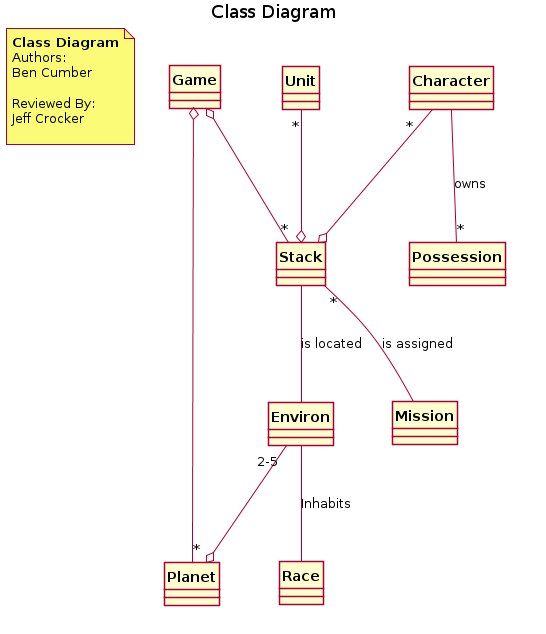
\includegraphics[width=6in,height=10in]{class_overview.png}
\newpage
A more complete diagram is found below, which includes member variables and the major, high level functions integrated into each class:
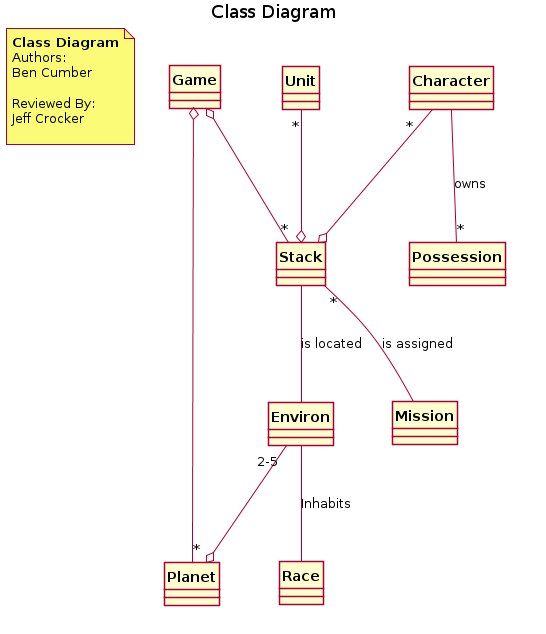
\includegraphics[width=6in,height=10in]{class_overview.png}
\newpage

\subsection[USER{\textquoteright}S ARCHITECTURAL
VIEW]{\selectlanguage{english}\bfseries\color{black}
USER{\textquoteright}S ARCHITECTURAL VIEW}
The only view that the user will have of this software is the view of the client. It is a graphical representation of the state of the game.

\subsubsection{User{\textquoteright}s View Identification}

{\selectlanguage{english}\color{black}
[Insert text here.]}

\subsubsection{User{\textquoteright}s View Representation and
Description }
{\selectlanguage{english}\itshape\color{black}
Provide a diagram and description of the user{\textquoteright}s view of
the architecture.}

{\selectlanguage{english}\color{black}
[Insert diagram here.]}

\subsection[Developer{\textquoteright}s View
Identification]{\selectlanguage{english}\bfseries\color{black}
Developer{\textquoteright}s View Identification}
{\selectlanguage{english}\itshape\color{black}
Identify the view, state the purpose of the view, and identify major
components or processes of the architecture.}

{\selectlanguage{english}\color{black}
The major overlaying architecture for this project relies on a client-server relation. In the case of the user, the client will consist of a player using a graphical interface to request and interact with the server. The client may also come in the form of the described AI, which makes the same types and formats of requests to the server. In this implementation, the server operates as the 'rule book' and authority on game state. Discrepancies in the game state will thus always defer to the records of the server. A typical example of this interaction would involve a client, player or AI, issuing a request (attempted move or game state update) and the server responding in turn, which notifies the client if the request resulted in success or failure, and updates the game state.}}

\subsubsection[Developer{\textquoteright}s View Representation and
Description ]{Developer{\textquoteright}s View Representation and
Description }
{\selectlanguage{english}\itshape\color{black}
Provide a diagram and description of the developer{\textquoteright}s
view of the architecture.}

{\selectlanguage{english}\color{black}
[Insert diagram here.]}

\subsubsection{Developer{\textquoteright}s Architectural Rationale}
{\selectlanguage{english}\itshape\color{black}
For compliance with ISO/IEC 42010:2007 (�5.6) an Architectural
Description (AD) shall provide the rationale that justified the
architect{\textquoteright}s decisions and selected architectures. An AD
shall also provide evidence of the consideration of other alternative
architectures and the rationales for discarding them.}

{\selectlanguage{english}\color{black}
[Insert rationale here.]}

\subsection[\ [ insert name of viewpoint {]} ARCHITECTURAL
VIEW]{\foreignlanguage{english}{\ }\foreignlanguage{english}{[ insert
name of viewpoint ] ARCHITECTURAL VIEW}}
{\selectlanguage{english}\itshape\color{black}
This subsection contains the descriptions of a system and all of its
major components, using the methods, techniques, and languages from
other than the developer{\textquoteright}s or user{\textquoteright}s
viewpoint. \ Each viewpoint description includes the viewpoint
identification, description, and diagrammatic representation. }


\bigskip

{\selectlanguage{english}\itshape\color{black}
Repeat this subsection for each viewpoint identified.}

\subsubsection{[ insert name of viewpoint ]{\textquoteright}s View
Identification}
{\selectlanguage{english}\itshape\color{black}
Identify the view, state the purpose of the view, and identify major
components or processes of the architecture.}

{\selectlanguage{english}\color{black}
[Insert text here.]}

\subsubsection{[ insert name of viewpoint ]{\textquoteright}s View
Representation and Description }
{\selectlanguage{english}\itshape\color{black}
Provide a diagram of the developer{\textquoteright}s view of the
architecture.}

{\selectlanguage{english}\color{black}
[Insert diagram and descriptions here.]}

\subsection[CONSISTENCY OF ARCHITECTURAL
VIEWS]{\selectlanguage{english}\bfseries\color{black} CONSISTENCY OF
ARCHITECTURAL VIEWS}
{\selectlanguage{english}\itshape\color{black}
For compliance with ISO/IEC 42010:2007 (�5.5) an Architectural
Description (AD) shall include a list of all known inconsistencies
between the architectural views and an analysis of consistency across
all the architectural views.}

\subsubsection{Detail of Inconsistencies between Architectural Views}
{\selectlanguage{english}\color{black}
[Insert text and graphics here.]}

\subsubsection{Consistency Analysis and Inconsistency Mitigations}
{\selectlanguage{english}\itshape\color{black}
For each inconsistency identified above, provide solutions or
mitigations that resolve potential conflicts between the stakeholder
viewpoints.}

{\selectlanguage{english}\color{black}
[Insert text or table here.]}

\section{SOFTWARE DETAILED DESIGN}
{\selectlanguage{english}\itshape\color{black}
This section of the document should describe with detail the design of
the software being described in this document. \ The level of detail of
the design entities and their relationship and interfaces shall be
sufficient to enable software implementers to implement an integrate
each of the described components in order to achieve full
implementation of the software being described in this SSDD. This
section shall specify for each design entity the following information:
purpose, processing, data, interfaces, dependencies and relationships,
concept of execution, needed resources, design rationale, information
for reuse, types of errors, and error handling. \ }


\bigskip

{\selectlanguage{english}\itshape\color{black}
The detailed design must correspond to an existing architectural view,
normally the developer{\textquoteright}s view, but unusual
circumstances may call for other detailed design viewpoints. \ If so,
repeat this subsection as needed for those other viewpoints.}

\subsection[\ DEVELOPER{\textquoteright}S VIEWPOINT DETAILED SOFTWARE
DESIGN]{\foreignlanguage{english}{\ }\foreignlanguage{english}{DEVELOPER{\textquoteright}S
VIEWPOINT DETAILED SOFTWARE DESIGN}}
{\selectlanguage{english}\itshape\color{black}
Identify the viewpoint and make reference to the diagram or model
defining the view.}

{\selectlanguage{english}\color{black}
[Insert text, diagram or model here.]}

\subsection[COMPONENT/ENTITY
DICTIONARY]{\selectlanguage{english}\bfseries\color{black}
COMPONENT/ENTITY DICTIONARY}
{\selectlanguage{english}\itshape\color{black}
This subsection shall list and describe all the detailed design entities
and their corresponding attributes. \ Processing and algorithms, data
and data structures,and detailed descriptions need NOT be included
here, as they will be specified in subsequent sections for each
component or entity listed in the table below.}

\begin{flushleft}
\tablehead{}
\begin{supertabular}{|m{1.0462599in}|m{0.9837598in}|m{1.6712599in}|m{1.2962599in}|m{1.2580599in}|}
\hline
\multicolumn{5}{|m{6.57056in}|}{\centering
\selectlanguage{english}\bfseries\color{black} Component/Entity
Dictionary}\\\hline
\centering \selectlanguage{english}\bfseries\color{black} Name &
\centering \selectlanguage{english}\bfseries\color{black} Type/Range &
\centering \selectlanguage{english}\bfseries\color{black}
Purpose/Function &
\centering \selectlanguage{english}\bfseries\color{black} Dependencies &
\centering\arraybslash \selectlanguage{english}\bfseries\color{black}
Subordinates\\\hline
~
 &
~
 &
~
 &
~
 &
~
\\\hline
~
 &
~
 &
~
 &
~
 &
~
\\\hline
~
 &
~
 &
~
 &
~
 &
~
\\\hline
~
 &
~
 &
~
 &
~
 &
~
\\\hline
~
 &
~
 &
~
 &
~
 &
~
\\\hline
\end{supertabular}
\end{flushleft}
\subsection[COMPONENT/ENTITY DETAILED
DESIGN]{\selectlanguage{english}\bfseries\color{black} COMPONENT/ENTITY
DETAILED DESIGN}
\subsubsection{Detailed Design for Component/Entity: [ insert
Component/Entity name here ]}
\paragraph[\ Introduction/Purpose of this
Component/Entity]{\ Introduction/Purpose of this Component/Entity}
{\selectlanguage{english}\color{black}
[ insert your text here ]}

\paragraph[Input for this Component/Entity]{Input for this
Component/Entity}
{\selectlanguage{english}\color{black}
[ insert your text here ]}

\paragraph{Output for this Component/Entity}
{\selectlanguage{english}\color{black}
[ insert your text here ]}

\paragraph{Component/Entity Process to Convert Input to Output}
{\selectlanguage{english}\color{black}
[ insert your text here ]}

\paragraph{Design constraints and performance requirements of this
Component/Entity}
{\selectlanguage{english}\color{black}
[ insert your text here ]}

\subsubsection{Detailed Design for Component/Entity: [ insert
Component/Entity name here ]}
\paragraph[\ Introduction/Purpose of this
Component/Entity]{\ Introduction/Purpose of this Component/Entity}
{\selectlanguage{english}\color{black}
[ insert your text here ]}

\paragraph{Input for this Component/Entity}
{\selectlanguage{english}\color{black}
[ insert your text here ]}

\paragraph{Output for this Component/Entity}
{\selectlanguage{english}\color{black}
[ insert your text here ]}

\paragraph{Component/Entity Process to Convert Input to Output}
{\selectlanguage{english}\color{black}
[ insert your text here ]}

\paragraph{Design constraints and performance requirements of this
Component/Entity}
{\selectlanguage{english}\color{black}
[ insert your text here ]}

\subsubsection{Detailed Design for Component/Entity: [ insert
Component/Entity name here ]}
\paragraph[\ Introduction/Purpose of this
Component/Entity]{\ Introduction/Purpose of this Component/Entity}
{\selectlanguage{english}\color{black}
[ insert your text here ]}

\paragraph{Input for this Component/Entity}
{\selectlanguage{english}\color{black}
[ insert your text here ]}

\paragraph{Output for this Component/Entity}
{\selectlanguage{english}\color{black}
[ insert your text here ]}

\paragraph{Component/Entity Process to Convert Input to Output}
{\selectlanguage{english}\color{black}
[ insert your text here ]}

\paragraph{Design constraints and performance requirements of this
Component/Entity}
{\selectlanguage{english}\color{black}
[ insert your text here ]}

\subparagraph[{\dots}]{{\dots}}
\subsubsection{Detailed Design for Component/Entity: [ insert
Component/Entity name here ]}
\paragraph[\ Introduction/Purpose of this
Component/Entity]{\ Introduction/Purpose of this Component/Entity}
{\selectlanguage{english}\color{black}
[ insert your text here ]}

\paragraph{Input for this Component/Entity}
{\selectlanguage{english}\color{black}
[ insert your text here ]}

\paragraph{Output for this Component/Entity}
{\selectlanguage{english}\color{black}
[ insert your text here ]}

\paragraph{Component/Entity Process to Convert Input to Output}
{\selectlanguage{english}\color{black}
[ insert your text here ]}

\paragraph{Design constraints and performance requirements of this
Component/Entity}
{\selectlanguage{english}\color{black}
[ insert your text here ]}

\subsection{DATA DICTIONARY}
{\selectlanguage{english}\itshape\color{black}
This subsection shall list and describe all the data and data structures
defined and/or used by the components and entities specified above.
\ For each data item or structure indicate where it is defined,
referenced, and modified.}

\begin{flushleft}
\tablehead{}
\begin{supertabular}{|m{0.9837598in}|m{0.9212598in}|m{1.8587599in}|m{1.2962599in}|m{1.1330599in}|}
\hline
\multicolumn{5}{|m{6.50806in}|}{\centering
\selectlanguage{english}\bfseries\color{black} Data Dictionary}\\\hline
\centering \selectlanguage{english}\bfseries\color{black} Name &
\centering \selectlanguage{english}\bfseries\color{black} Type/Range &
\centering \selectlanguage{english}\bfseries\color{black} Defined
by{\dots} &
\centering \selectlanguage{english}\bfseries\color{black} Referenced
by{\dots} &
\centering\arraybslash \selectlanguage{english}\bfseries\color{black}
Modified by{\dots}\\\hline
~
 &
~
 &
~
 &
~
 &
~
\\\hline
~
 &
~
 &
~
 &
~
 &
~
\\\hline
~
 &
~
 &
~
 &
~
 &
~
\\\hline
~
 &
~
 &
~
 &
~
 &
~
\\\hline
~
 &
~
 &
~
 &
~
 &
~
\\\hline
\end{supertabular}
\end{flushleft}

\bigskip


\bigskip

\clearpage\setcounter{page}{1}\pagestyle{Convertvii}
\section[REQUIREMENTS
TRACEABILITY]{\selectlanguage{english}\bfseries\color{black}
REQUIREMENTS TRACEABILITY}
{\selectlanguage{english}\color{black}
\foreignlanguage{english}{\textit{This section shall contain
traceability information from each system requirement in this
specification to the system (or subsystem, if applicable) requirements
it addresses. \ A tabular form is preferred, but not mandatory.
}}\foreignlanguage{english}{\textit{A detailed mapping between
requirements and constraints in the SSRS and architectural components
and detailed entities in this SSDD is required. For compliance with
ISO/IEC 15288:2008
}}\foreignlanguage{english}{\textit{(�6.4.3.3.c)}}\foreignlanguage{english}{\textit{
an Architectural Description (AD) shall provide roundtrip traceability
between the system and software requirements and the architectural
design entities. All requirements and constraints within the SSRS shall
map to a set of architectural entities. All entities in all the
architectural views shall be associated with either a requirement or
constraint in the SSRS or an architectural constraint within this
SSDD.}}}


\bigskip

\begin{flushleft}
\tablehead{\hline
\multicolumn{1}{|m{0.9212598in}|}{\centering
\selectlanguage{english}\bfseries\color{black} Feature Name} &
\centering \selectlanguage{english}\bfseries\color{black} Req No. &
\centering \selectlanguage{english}\bfseries\color{black} Requirement
Description &
\centering \selectlanguage{english}\bfseries\color{black} Priority &
\centering \selectlanguage{english}\bfseries\color{black} SDD &
\multicolumn{2}{m{1.2872598in}|}{\centering
\selectlanguage{english}\bfseries\color{black} Alpha Release} &
\multicolumn{2}{m{1.3587599in}|}{\centering
\selectlanguage{english}\bfseries\color{black} Beta Release} &
\multicolumn{2}{m{1.3795599in}|}{\centering
\selectlanguage{english}\bfseries\color{black} Final Test}\\\hline
 &
 &
 &
 &
 &
\centering \selectlanguage{english}\bfseries\color{black} Test Case(s) &
\centering \selectlanguage{english}\bfseries\color{black} Test Res. &
\centering \selectlanguage{english}\bfseries\color{black} Test Case(s) &
\centering \selectlanguage{english}\bfseries\color{black} Test Res. &
\centering \selectlanguage{english}\bfseries\color{black} Test Case(s) &
\selectlanguage{english}\bfseries\color{black} Test
Res.\\\hhline{~~~~~------}}
\begin{supertabular}{m{0.9212598in}|m{0.42125985in}|m{1.9212599in}|m{0.39275986in}|m{0.7587598in}|m{0.6622598in}|m{0.5462598in}|m{0.6712598in}|m{0.6087598in}|m{0.6712598in}|m{0.6295598in}|}
\multicolumn{1}{|m{0.9212598in}|}{~
} &
\centering \selectlanguage{english}\color{black} 1.1 &
~
 &
~
 &
~
 &
~
 &
~
 &
~
 &
~
 &
~
 &
~
\\\hline
 &
\centering \selectlanguage{english}\color{black} 1.2 &
~
 &
~
 &
~
 &
~
 &
~
 &
~
 &
~
 &
~
 &
~
\\\hhline{~----------}
 &
\centering \selectlanguage{english}\color{black} {\dots} &
~
 &
~
 &
~
 &
~
 &
~
 &
~
 &
~
 &
~
 &
~
\\\hhline{~----------}
 &
\centering \selectlanguage{english}\color{black} 1.[n] &
~
 &
~
 &
~
 &
~
 &
~
 &
~
 &
~
 &
~
 &
~
\\\hhline{~----------}
\multicolumn{1}{|m{0.9212598in}|}{~
} &
\centering \selectlanguage{english}\color{black} 2.1 &
~
 &
~
 &
~
 &
~
 &
~
 &
~
 &
~
 &
~
 &
~
\\\hline
 &
\centering \selectlanguage{english}\color{black} 2.2 &
~
 &
~
 &
~
 &
~
 &
~
 &
~
 &
~
 &
~
 &
~
\\\hhline{~----------}
 &
\centering \selectlanguage{english}\color{black} {\dots} &
~
 &
~
 &
~
 &
~
 &
~
 &
~
 &
~
 &
~
 &
~
\\\hhline{~----------}
 &
\centering \selectlanguage{english}\color{black} 2.[n] &
~
 &
~
 &
~
 &
~
 &
~
 &
~
 &
~
 &
~
 &
~
\\\hhline{~----------}
\multicolumn{1}{|m{0.9212598in}|}{~
} &
\centering \selectlanguage{english}\color{black} 3.1 &
~
 &
~
 &
~
 &
~
 &
~
 &
~
 &
~
 &
~
 &
~
\\\hline
 &
\centering \selectlanguage{english}\color{black} 3.2 &
~
 &
~
 &
~
 &
~
 &
~
 &
~
 &
~
 &
~
 &
~
\\\hhline{~----------}
 &
\centering \selectlanguage{english}\color{black} {\dots} &
~
 &
~
 &
~
 &
~
 &
~
 &
~
 &
~
 &
~
 &
~
\\\hhline{~----------}
 &
\centering \selectlanguage{english}\color{black} 3.[n] &
~
 &
~
 &
~
 &
~
 &
~
 &
~
 &
~
 &
~
 &
~
\\\hhline{~----------}
\multicolumn{1}{|m{0.9212598in}|}{\selectlanguage{english}\color{black}
{\dots}} &
\centering \selectlanguage{english}\color{black} {\dots} &
~
 &
~
 &
~
 &
~
 &
~
 &
~
 &
~
 &
~
 &
~
\\\hline
\multicolumn{1}{|m{0.9212598in}|}{~
} &
\centering \selectlanguage{english}\color{black} [m].1 &
~
 &
~
 &
~
 &
~
 &
~
 &
~
 &
~
 &
~
 &
~
\\\hline
 &
\centering \selectlanguage{english}\color{black} [m].2 &
~
 &
~
 &
~
 &
~
 &
~
 &
~
 &
~
 &
~
 &
~
\\\hhline{~----------}
\multicolumn{1}{|m{0.9212598in}|}{~
} &
\centering \selectlanguage{english}\color{black} {\dots} &
~
 &
~
 &
~
 &
~
 &
~
 &
~
 &
~
 &
~
 &
~
\\\hline
\multicolumn{1}{|m{0.9212598in}|}{~
} &
\centering \selectlanguage{english}\color{black} [m.n] &
~
 &
~
 &
~
 &
~
 &
~
 &
~
 &
~
 &
~
 &
~
\\\hline
\end{supertabular}
\end{flushleft}
{\selectlanguage{english}\color{black}
Priorities are: \textbf{M}andatory, \textbf{L}ow, \textbf{H}igh}

{\selectlanguage{english}\color{black}
SDD link is version and page number or function name.}

{\selectlanguage{english}\color{black}
Test cases and results are file names and \textbf{P}ass/\textbf{F}ail or
\% passing.}

\clearpage\setcounter{page}{1}\pagestyle{Convertviii}
\section[APPENDIX A. \ [insert name
here{]}]{\selectlanguage{english}\bfseries\color{black} APPENDIX A.
\ [insert name here]}
{\selectlanguage{english}\itshape\color{black}
Include copies of specifications, mockups, prototypes, etc. supplied or
derived from the customer. \ Appendices are labeled A, B, {\dots}n.
\ \ Reference each appendix as appropriate in the text of the document.
}

{\selectlanguage{english}\color{black}
\ [ insert appendix A here ]}

\clearpage\setcounter{page}{1}\pagestyle{Convertix}
\section[APPENDIX B. \ [insert name
here{]}]{\selectlanguage{english}\bfseries\color{black} APPENDIX B.
\ [insert name here]}

\bigskip

{\selectlanguage{english}\color{black}
[ insert appendix B here ]}


\bigskip
\end{document}
